\documentclass[12pt, french]{report}

\usepackage[top=3cm, bottom=3cm, left=3cm, right=3cm]{geometry}
\usepackage[T1]{fontenc}
\usepackage[utf8]{inputenc}
\usepackage{babel}
\usepackage{graphicx}
\usepackage{hyperref}
\usepackage{pdfpages}
\usepackage{gensymb}
\usepackage{eurosym}
\usepackage{xcolor}
% \usepackage{appendix}
\usepackage{amsmath,amsfonts,amssymb}
\usepackage{float}                % needed for floating figure
\usepackage[toc,xindy]{glossaries}

\hypersetup{                      % parametrage des hyperliens
  colorlinks=true,                % colorise les liens
  breaklinks=true,                % permet les retours à la ligne pour les liens trop longs
  urlcolor= blue,                 % couleur des hyperliens
  linkcolor= blue,                % couleur des liens internes aux documents
  citecolor= green                % couleur des liens vers les references bibliographiques
}

\makeglossaries

\newglossaryentry{devops}
{
  name=DevOps,
  description={Pratique technique visant à l'unification du développement logiciel (dev) et de l'administration des infrastructures informatiques (ops)}
}

\newglossaryentry{nosql}
{
  name=NoSQL,
  description={Famille de systèmes de gestion de base de données}
}

\newglossaryentry{hadoop}
{
  name=Hadoop,
  description={Framework libre et open source écrit en Java destiné à faciliter la création d'applications distribuées}
}

\newglossaryentry{sre}
{
  name=SRE,
  description={Discipline qui intègre des aspects de l'ingénierie logicielle et les applique aux problèmes d'infrastructure et d'exploitation}
}

\newglossaryentry{paas}
{
  name=PAAS,
  description={Platform as a service (Plate-forme en tant que service) - Types de cloud computing où le fournisseur cloud maintient la plate-forme d'exécution des applications}
}

\newglossaryentry{github}
{
  name=GitHub,
  description={Service web d'hébergement et de gestion de développement de logiciels, utilisant le logiciel de gestion de versions \gls{git}}
}

\newglossaryentry{git}
{
  name=Git,
  description={Logiciel libre de gestion de versions décentralisé}
}

\newglossaryentry{nodejs}
{
  name=Node.js,
  description={Plateforme logicielle libre en \gls{javascript} orientée vers les applications réseau événementielles}
}

\newglossaryentry{javascript}
{
  name=JavaScript,
  description={Langage de programmation de scripts principalement employé dans les pages web interactives mais aussi pour les serveurs}
}

\begin{titlepage}
\title{	
\includegraphics[scale=0.4]{assets/img/logo-adaltas.png}\\[1 cm]
		\normalsize \textsc{Rapport de stage}\\[0.8cm]
		{Entreprise partenaire : \\Adaltas}\\[0.8 cm]
		\rule{\linewidth}{0.2 mm} \\[0.4 cm]
		\LARGE \textbf{\uppercase{Mise en place d'une solution d'automatisation pour le déploiement de sysèmes Big Data}}
		\rule{\linewidth}{0.2 mm}
		}
\author {\normalsize Auteur :\\	\normalsize Alexander Hoffmann - alexander@adaltas.com\\[0.5 cm]
		 \normalsize Maître de stage :\\	\normalsize David Worms - david@adaltas.com\\}
\date{\normalsize \today}
\end{titlepage}

\begin{document}
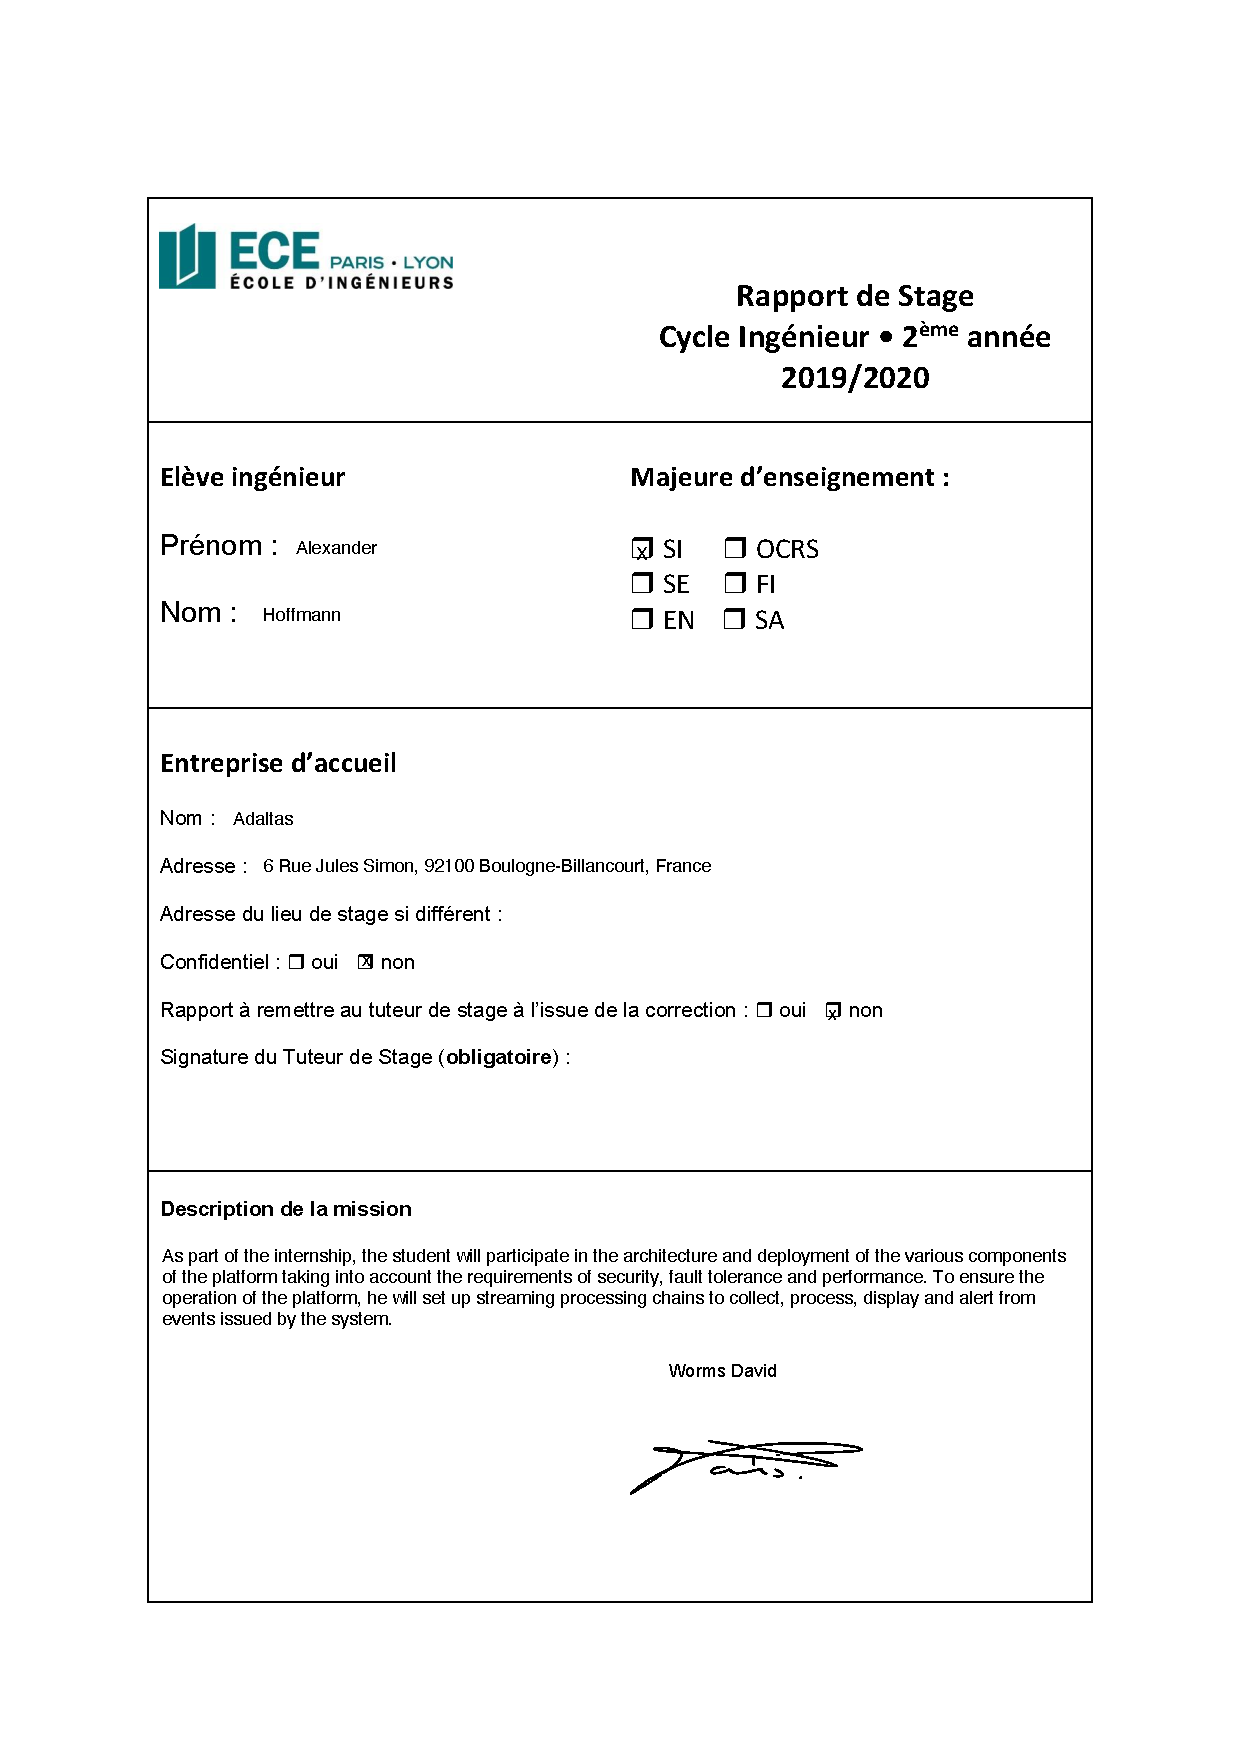
\includepdf[pages=-]{assets/pdf/title.pdf}

\maketitle

\chapter*{Remerciements}

Les premiers pas dans le monde du travail se font rarement seul et sans aide ni soutien. Je souhaite remercier toutes les personnes ayant contribué à cette expérience professionnelle.\\

Je tiens tout d’abord à remercier toute l'équipe d'Adaltas pour son accueil, sa bienveillance et sa bonne humeur permanente. J'apprécie l'attention et la sollicitude qui m'ont été prodiguées par toute personne rencontrée.\\

Je voudrais ensuite exprimer ma sincère gratitude à David Worms, mon tuteur, pour la confiance qu’il a bien voulu m’accorder en acceptant de m'intégrer à Adaltas. Je le remercie pour sa grande disponibilité, sa patience, son soutien chaleureux et ses conseils avisés. Je tiens à lui exprimer ma profonde reconnaissance pour ses critiques constructives d’une rigueur absolue.\\

Mes remerciements s’adressent également à Prisca Borges pour son accueil, sa sympathie et ses conseils, ainsi qu'à Léo Schoukroun pour son encadrement et sa compréhension qu'il m'a accordé tout au long du stage.\\

En cette période inédite de crise sanitaire, j'ai eu la chance de pouvoir travailler avec une entreprise qui a su s'adapter aux difficultés posées par les mesures nécessaires à la protection de ses collaborateurs. Je suis reconnaissant d'avoir pu effectuer mon stage dans les meilleurs conditions possibles.

\chapter*{Résumé}

Ce document décrit mon stage de 2ème année du cycle ingénieur effectué au sein de l'entreprise Adaltas. Adaltas est une équipe de consultants experts en Open Source, Big Data et systèmes distribués. La société fournit à ses clients un savoir faire reconnu sur la manière d'utiliser les technologies pour convertir leurs cas d'usage en projets exploités en production, sur la façon de réduire les coûts et d'accélérer les livraisons de nouvelles fonctionnalités.\\

Au sein de cette structure, j'ai eu la chance d'évoluer en tant que développeur. J'ai travaillé sur Nikita\footnote{\href{https://github.com/adaltas/node-nikita}{https://github.com/adaltas/node-nikita}}, une librairie d’automatisation pour le déploiement de systèmes pour \gls{nodejs}. Ce logiciel a été conçu dans le but d'aider les développeurs et les opérateurs à déployer des infrastructures et des logiciels Big Data de manière flexible et idempotente.\\

L'objectif de ce stage était de contribuer au développement d'un projet Open Source et ainsi d'en apprendre plus sur cet axe de valorisation. Adaltas est une société “open”. Son engagement se construit sur les fondations d’un code source ouvert, d’une collaboration ouverte, de standards ouverts et d’une formation ouverte. Il s'agit d'une façon de penser et de travailler à laquelle j'adhère fortement. C'est également l'une des raisons pour lesquelles j'ai choisi d'effectuer mon stage chez Adaltas.\\

\noindent\textbf{Mots clés} : big data, déploiement, devops, infraops.

\begingroup
\hypersetup{linkcolor=black}
\listoffigures
\tableofcontents
\newpage
\endgroup

\chapter*{Introduction}
\addcontentsline{toc}{chapter}{Introduction}

Mon intérêt pour la data science et plus généralement pour l’informatique et les nouvelles technologies m’ont amené à chercher un stage dans une société qui en a fait son coeur de métier. Le début de ma recherche de stage a été le mois de juillet 2019. J'ai envoyé des candidatures à plus d'une centaine d'entreprise dont Google, Amazon, Facebook et Apple. J'ai eu la chance de passer des entretiens techniques chez trois des entreprises citées précédemment. Sans trop entrer dans les détails, les épreuves comportent des questions algorithmiques appliquées à des problèmes ludiques qu'il s'agit de résoudre dans une durée impartie. Florent Diedler, un enseignant en informatique à l'ECE, m'a d'ailleurs beaucoup aidé lors de la préparation à ces entretiens. N'ayant eu aucune proposition de stage, j'ai continué mes recherches.\\

C'est durant un cours de \gls{devops} animé par Gregor Jouet, consultant chez Adaltas, que j'ai découvert cette entreprise, ses méthodologies et sa culture. Aux alentours du mois de novembre, alors que nous travaillions sur un projet \gls{devops}, Gregor Jouet a invité les élèves intéressées par les technologies data science et big data à envoyer lui envoyer leur CV. Quelques semaines plus tard, j'ai reçu un appel de David Worms, dirigeant de la société Adaltas, qui m'a proposé un entretien.\\

Ce document présente les travaux et missions effectués au sein de l'entreprise Adaltas durant mon stage se déroulant du 14 avril au 30 août 2020, ceci représentant une durée totale de 4 mois et demi. Dans le cadre du stage, j'ai pu participer à l’architecture et au déploiement des différents composants d'un cluster en prenant en compte les impératifs de sécurité, de tolérance aux pannes et de performances. Pour assurer l’exploitation de la plateforme, j'ai mis en place des chaînes de traitement en streaming pour collecter, traiter, afficher et alerter à partir des évènements émis par le système.\\

La thématique de ce stage s’inscrit dans un contexte d’appréhension et d'approfondissement du monde de l’entreprise. Dans ce rapport, nous présenterons dans un premier temps le contexte du stage, c’est-à-dire que nous décrirons l’entreprise d’accueil, nous étudierons son secteur d’activité et sa culture. Dans un second temps, nous expliquerons les différents aspects de ma mission et les attentes de l'entreprise. Finalement, nous verrons les compétences et qualités acquises sur cette mission ainsi que ma valeur ajoutée pour l'entreprise.

\chapter{Présentation de la structure d'accueil: Adaltas}

Fondée en 2004, Adaltas est une société d’expertise en High Tech construite à partir de deux idées :
\begin{itemize}
  \item[--] l’innovation comme facteur de différenciation décisif pour les entreprises;
  \item[--] la capacité à mobiliser les meilleurs talents comme condition de succès.\\
\end{itemize}

\begin{figure}[H]

\includegraphics[scale=0.4]{assets/img/logo-adaltas.png}
\centering
\caption{Logo d'Adaltas représentant un oiseau. Adaltas signifie "vers le haut".}
\label{fig:logo-adaltas}
\end{figure}

Adaltas aide ses clients à s’orienter dans le monde en perpétuelle évolution de l’Open Source, leur donnant les clés pour développer les meilleures solutions, qu’il s’agisse simplement d’écrire une application ou d’élaborer une plateforme de traitement stratégique à plus long terme. L'entreprise se définit comme un acteur du Big Data autour des technologies \gls{hadoop} et \gls{nosql}.

Les équipes apportent une expertise sur l’analyse et le traitement des données, leur gouvernance, le développement et la gestion opérationnelle. Les consultants adhèrent à la culture \gls{devops} et ils sont formés à la méthodologie \gls{sre}\footnote{\href{https://landing.google.com/sre/}{What is Site Reliability Engineering (SRE)?}}. Ils accompagnent leur client dans la mise en place d’infrastructures et d’applications résilientes, conscients des rapides innovations apportés par la communauté Open Source et de la nécessaire stabilité des systèmes.

L'expertise d'Adaltas dans le domaine Big Data a commencé dès 2009 par l'accompagnement de la société EDF et la collecte des données Linky dit compteurs intelligents. En 2012, la société a entrepris l’exploitation d'une plateforme commune à l'ensemble du groupe EDF avec la mise à disposition des composants de l’éco-système Hadoop. Le nombre de composants s'est élargi avec le temps ainsi que les services et les cas d’usage qui ont accosté sur la plateforme sécurisé et multi-tenante.

Depuis 2014, l’équipe s’est élargie en accueillant des talents majoritairement formés à l’ECE, école dans laquelle Adaltas est à l’initiative du programme Big Data. Adaltas donne également des cours au Data Science Tech Institute\footnote{\href{https://www.datasciencetech.institute/}{https://www.datasciencetech.institute/}} et à l’Université Paris-Sorbonne. La société cherche à recruter et former ses futurs consultants le plus tôt possible afin qu'ils soient opérationnels dès la fin du stage de dernière année d'école.

\section{Objectifs de l'entreprise}

L’acquisition d’un cluster à forte capacité répond à la volonté d’Adaltas de construire une offre de type \gls{paas} pour disposer et mettre à disposition des plateformes de Big Data et d’orchestration de conteneurs. Les plateformes sont utilisées pour l’acquisition de nouvelles compétences, l’évaluation de nouvelles technologies, l’utilisation d’outils \gls{devops} et la mise à disposition d’environnements de développement, de PoCs et d’exploitation. Elles hébergent des Data Lakes, des DataLabs, des traitements et des modèles de Data Science, des outils orientés \gls{devops} ou encore des services applicatifs. L’objectif est de porter cette offre à maturité.

\section{Une entreprise "open"}

Adaltas est une société “open”. Leur engagement se construit sur les fondations d’un code source ouvert, d’une collaboration ouverte, de standards ouverts et d’une formation ouverte.

Les entreprises et les gouvernements utilisent les technologies Open Source pour remplacer les solutions propriétaires. Initialement, ces acteurs ont été attirés par les réductions de coût et la promesse de s’affranchir de la dépendance d’un éditeur. L’Open Source est désormais central à la transformation digitale avec des avantages avérés dans la sécurité, la qualité, la personnalisation, la flexibilité, l’intéropérabilité, l’auditabilité et le soutien.

Adaltas maintient près de 50 dépôts Open Source sur \gls{github} et encourage chaque développeur et client à contribuer à ces projets.

\chapter{Présentation de la mission}

Cette partie décrit les activités réalisées dans le cadre du stage. La plupart d'entre elles ont été réalisées en parallèle. La description "chronologique" qui suit est donc très relative.

\section{Cahier des charges}

Sur la base des différents objectifs présentés précédemment, un cahier des charges a été établi mi-avril 2020 par David Worms. Les activités précisées sont les suivantes : 

\begin{enumerate}
  \item Refactoring du code source du package \texttt{engine} afin d'en améliorer la lisibilité et, par voie de conséquence, la maintenance, et à le rendre plus générique.
  \item Migration des actions du module \texttt{file}, initialement contenue dans le package \texttt{core}, vers son propre package.
  \item Amélioration de la documentation dans les packages \texttt{engine} et \texttt{file} dans le but de la rendre plus complète et compréhensible.
  \item Conception de tests unitaires permettant de vérifier le bon fonctionnement des packages \texttt{engine} et \texttt{file}.
  \item Délivrance d'un rapport de stage à l'ECE Paris et à Adaltas.
\end{enumerate}

\section{Planning}

  Le découpage temporel des missions proposé au début du stage est décrit sur la figure \ref{fig:planning}. Ce planning a été formulé en fonction de ma progression prévisionnelle de l'apprentissage des technologies nécessaires au développement de Nikita. Lesdites technologies seront étudiées en détails ci-après.

\begin{figure}[h]
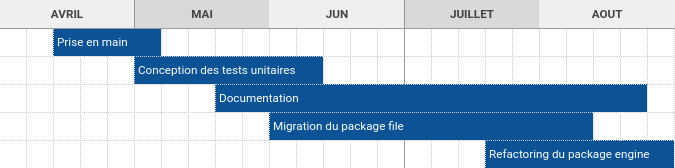
\includegraphics[scale=0.6]{assets/img/planning.png}
\centering
\caption{Planning sous forme de diagramme de Gantt}
\label{fig:planning}
\end{figure}

\section{Prise en main}

Ma première activité consistait à comprendre la logique de Nikita. Pour pouvoir m'approprier et faire évoluer ce logiciel, il me fallait tout d'abord comprendre sa manière de fonctionner.

\chapter*{Conclusion}
\addcontentsline{toc}{chapter}{Conclusion}

Fort des éléments énoncés précédemment, ce stage technique effectué au sein de l’entreprise Adaltas constitue une expérience des plus enrichissantes étant donné la complexité technique des missions auxquelles j'ai pu prétendre. Outre l’aventure humaine que j’eus la chance et le privilège de vivre, ce stage m’apprit le sens de la rigueur, du professionnalisme, ainsi que l’importance du temps et de son agencement. Grâce à cette expérience, j’ai acquis des compétences telles que le fonctionnement de (.................). De plus, les différentes missions effectuées m’ont permis d’accroître ma volonté de savoir et de connaissance, notamment dans le domaine du Big Data.

\clearpage

\printglossaries

\end{document}

